Pour l'instant, les visualisations ne sont que des preuves de concept mais nous pouvons envisager leur intégration future dans l'application AIKON. Il s'agit de recommandations qui ne seront pas nécessairement suivies par les membres de l'équipe lors de la conception des visualisations finales.

\subsection{Mise en place des visualisations}

\subsubsection{Emplacement sur la plateforme}

Pour intégrer les visualisations dans l'application, nous pourrions créer un nouvel onglet nommé \textit{Browse} en prenant exemple sur \gls{dishas}. Cet onglet comprendra deux sections, chacune correspondant à une visualisation : \textit{Pairs} pour le \textit{bipartite graph} et \textit{Network} pour le \textit{force-directed layout}. Il est également possible de les intégrer à un outil pour naviguer au sein des résultats du traitement automatique comme \textit{Explore} issu du projet \textit{Visual Contagion}. Nous pourrions appeler ce dernier \textit{DiscoViz}, la contraction entre les mots \textit{discover} et \textit{visualize}. Ces deux options donneraient à l'utilisateur la possibilité de comparer deux \textit{witnesses} avec le \textit{bipartite graph} ou plusieurs sous la forme de réseaux avec la visualisation \textit{force-directed layout}.

\begin{figure}[H]
	\centering
	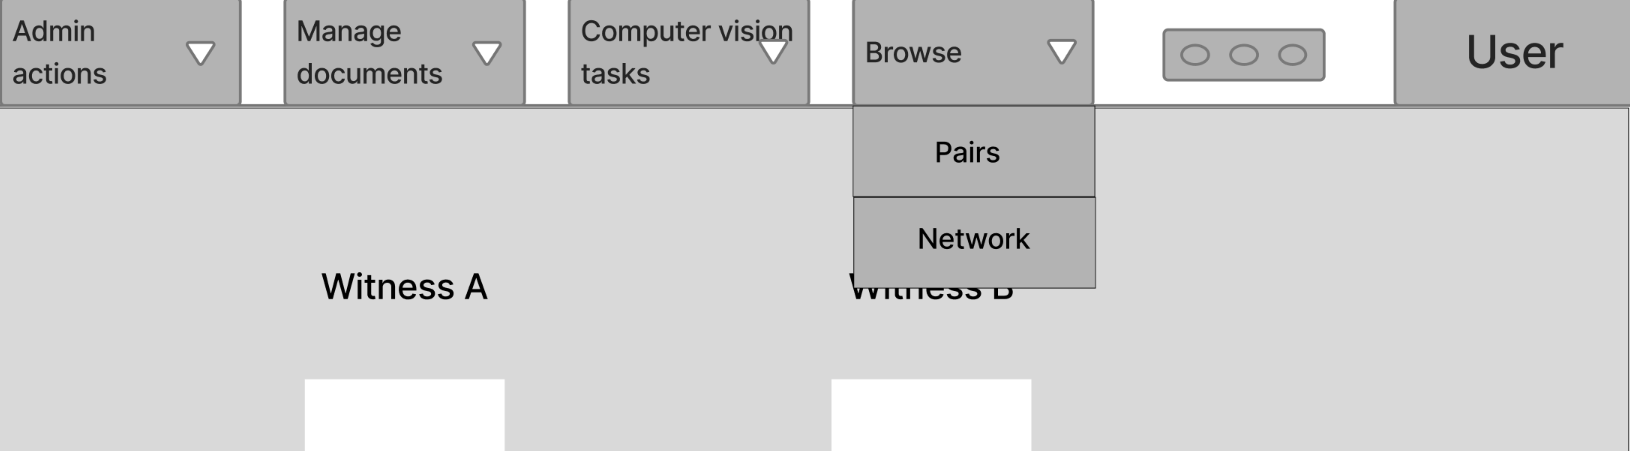
\includegraphics[width=0.6\textwidth]{images/barre_recherche_browse.png}
	\caption{Maquette représentant le nouvel onglet \textit{Browse}}
	\label{fig:browse}
\end{figure}

\begin{figure}[H]
	\centering
	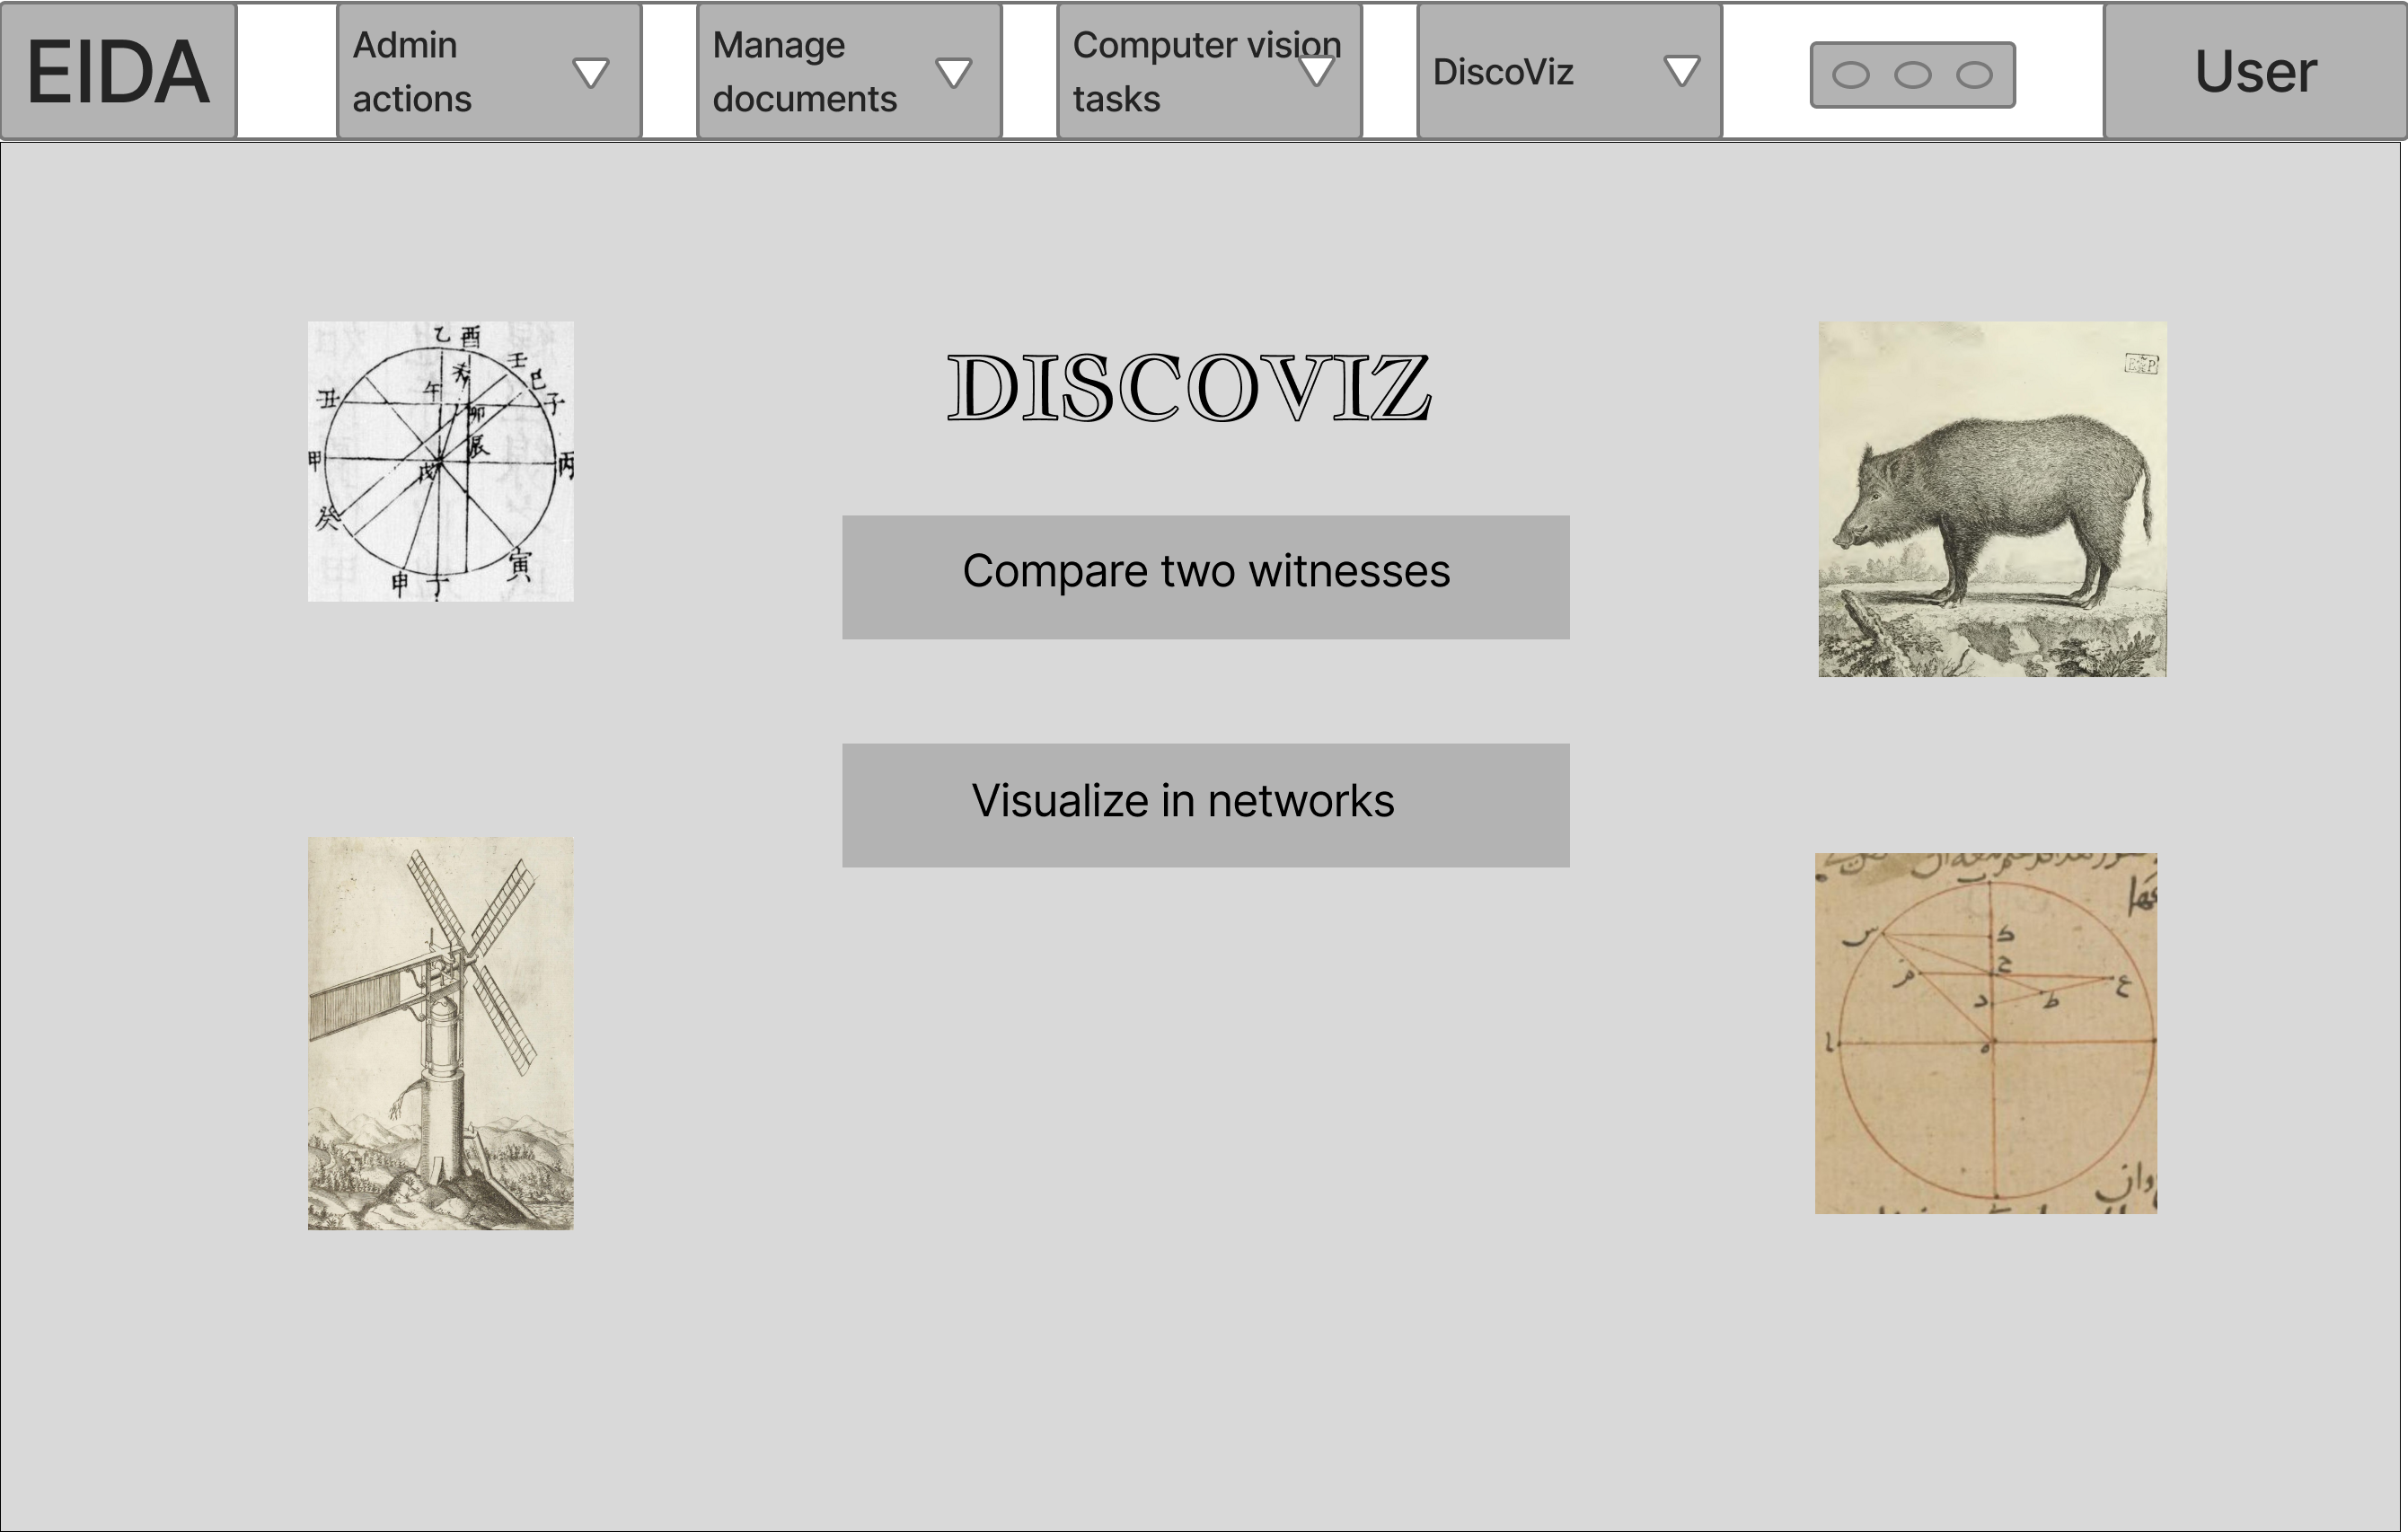
\includegraphics[width=0.8\textwidth]{images/maquette_discoviz.png}
	\caption{Maquette de la page d'accueil de l'outil \textit{DiscoViz}}
	\label{fig:discoviz}
\end{figure}

\subsubsection{La connexion à la base de données}

La transition de la preuve de concept vers l'intégration dans l'application nécessite une connexion à la base de données AIKON.
En effet, être dépendant de fichiers \gls{csv} ou \gls{gexf} n'aurait aucun intérêt puisque cette solution existe. 
De plus, il est nécessaire d'ajouter de nouvelles fonctionnalités comme celle du choix des \textit{witnesses} par le biais d'un menu déroulant ou d'une barre de recherche. Dans le cas de la visualisation \textit{force-directed layout}, il faut penser à ajouter un bouton \textit{+} pour sélectionner davantage de \textit{witnesses}.


\subsubsection{Technologies utilisées}

A présent, nous allons évoquer les outils numériques que nous pourrions utiliser afin d'ajouter les visualisations dans l'application. 

Puisque l'application AIKON est développée en Python à l'aide du \textit{framework} Django, la solution la plus simple est d'utiliser du \gls{html}, du \gls{css} et du JavaScript pour les intégrer aux \textit{templates}.

Pour le \textit{bipartite graph}, nous avons déjà créé la preuve de concept dans un document \gls{html} avec du \gls{css} et du JavaScript avec la bibliothèque D3.js. Il sera donc plus simple de l'intégrer dans l'application.

En ce qui concerne la visualisation \textit{force-directed layout}, il faudra la recoder entièrement car actuellement elle n'est visualisable que sur Gephi Lite. Nous pourrons utiliser la bibliothèque JavaScript Sigma.js évoquée précédemment. 

\subsubsection{Développement dans l'application}

Dans une application Django, nous devrons définir deux nouvelles routes dans \texttt{urls.py}. Il faudra également créer deux vues dans le fichier \texttt{views.py}. Ensuite, il sera nécessaire d'ajouter l'onglet supplémentaire à \texttt{base.html}. Pour finir, nous pourrons créer des \textit{templates} pour les visualisations.



\subsection{Perspectives non approfondies}

La durée du stage étant limitée, nous n'avons pas eu le temps de nous concentrer sur certains points importants en développement web comme le design et l'accessibilité dans l'élaboration des visualisations. 

\subsubsection{Le design}

La question du design est un point à ne pas négliger lorsque nous effectuons du développement web car cela a un impact sur l'expérience de l'utilisateur.

Le \gls{ui} concerne la conception visuelle et interactive d'une interface. Il prend donc en compte tous les choix liés à son apparence. Les visualisations sont concernées par ces décisions\footcite{snowebGuideLUIDesign}.

Durant le stage, nous n'avons pas eu le temps de nous focaliser sur le \gls{ui} des visualisations dans nos preuves de concept. Nous nous sommes limités à l'aspect fonctionnel des différents éléments. 

Pour réussir le \gls{ui} de nos visualisations, il faut d'abord s'attarder sur les couleurs et typographies. En effet, il est nécessaire de respecter la charte graphique pour obtenir un résultat harmonieux. Par exemple, les couleurs utilisées dans l'application AIKON sont plutôt dans les tons gris. Cela nous laisse la possibilité d'utiliser des couleurs un peu plus vives pour nos visualisations à condition de ne pas tomber dans l'exagération. Nous pouvons utiliser du rouge ou du bleu foncés pour les liens tout en prenant en compte le fait que la couleur des images dans les \textit{nodes} est plutôt claire. Au contraire, des tons trop clairs pourrait perturber la visibilité. Nous devons privilégier des polices d'écriture simples et épurées pour ne pas nuire à la lisibilité des éléments textuels. En ce qui concerne les \textit{labels} des \textit{nodes}, nous devons choisir une police simple et veiller à ce que la taille des lettres ne soit pas trop conséquente pour voir correctement les liens et les nœuds.

Autre point important : l'aspect des boutons. Dans la visualisation \textit{bipartite graph}, nous en avons ajouté un pour gérer le flux des données. Cependant, nous nous sommes contentés d'un bouton fonctionnel bleu qui n'est pas forcément très esthétique. Dans la version finale, il sera possible d'en ajouter un en harmonie avec l'aspect général de l'interface. Il est également possible de personnaliser la barre de chargement lorsque nous appuyons dessus en attendant que les images soient chargées. Nous pouvons aussi améliorer l'aspect de la \textit{check-box} pour afficher les scores de similarité, notamment en changeant la couleur du \textit{checkmark} afin de mieux adhérer à la charte graphique. 


\subsubsection{L'accessibilité}

Un point qui n'a pas encore été évoqué lors de la conception des visualisations est celle de l'accessibilité. Cette dernière a pour but de faciliter la navigation pour des personnes en situation de handicap cognitif, auditif ou visuel mais aussi moteur\footcite{QuestCeQue2025}.

Pour nous faciliter la tâche, nous pouvons nous appuyer sur le \gls{rgaa}\footcite{directioninterministerielledunumeriquedinumReferentielGeneralDamelioration2023} et le \gls{wcag}\footcite{w3cwebaccessibilityinitiativewaiReglesPourLaccessibilite} qui sont des référentiels définissant des règles et des bonnes pratiques pour l'accessibilité des sites web.

Rendre accessible des visualisations en réseaux est un véritable défi car il s'agit de représentations visuelles complexes. D'un point de vue visuel, il est important que le zoom ne déforme pas totalement la visualisation. Il faut également faire en sorte d'établir un contraste important au niveau des couleurs. Néanmoins, il faut prêter attention à ce que la couleur ne soit pas la seule manière de transmettre les informations. L'idéal serait d'avoir un contenu textuel alternatif à la visualisation pour décrire le nombre de nœuds, ceux avec le plus de liens et le nombre de relations\footcite{langeUltimateChecklistAccessible2024}. Certains types de police d'écriture sont plus adaptés que d'autres. Par exemple, la police d'écriture \textit{Luciole}, fruit d'une collaboration entre le Centre Technique Régional pour la Déficience Visuelle et le studio typographies.fr, a été spécialement conçue pour les personnes malvoyantes\footcite{centretechniqueregionalpourladeficiencevisuellectrdvtypographies.frLuciole2025}. Parfois une représentation statique est plus appropriée pour certains types de handicaps\footcite{langeUltimateChecklistAccessible2024}. Il faut également éviter les animations trop rapides pour les personnes épileptiques.

